%
% Common preamble for all three parts.
%
\usepackage[T1]{fontenc}
\usepackage[utf8]{inputenc}
\usepackage[catalan]{babel}
\usepackage{amsmath}
\usepackage{color}
\usepackage{minted}
\usepackage{hyperref}
\usepackage{multicol}
\usepackage{tabularx, booktabs}
\usepackage{tikz}

% only inline todonotes work
\usepackage{xkeyval}
\usepackage[textsize=small]{todonotes}
\presetkeys{todonotes}{inline}{}

\usetikzlibrary{shapes,arrows,positioning,shadows}

% no nav buttons
\usenavigationsymbolstemplate{}

\newcommand{\bftt}[1]{\textbf{\texttt{#1}}}
\newcommand{\comment}[1]{{\color[HTML]{008080}\textit{\textbf{\texttt{#1}}}}}
\newcommand{\cmd}[1]{{\color[HTML]{008000}\bftt{#1}}}
\newcommand{\bs}{\char`\\}
\newcommand{\cmdbs}[1]{\cmd{\bs#1}}
\newcommand{\lcb}{\char '173}
\newcommand{\rcb}{\char '175}
\newcommand{\cmdbegin}[1]{\cmdbs{begin\lcb}\bftt{#1}\cmd{\rcb}}
\newcommand{\cmdend}[1]{\cmdbs{end\lcb}\bftt{#1}\cmd{\rcb}}

\newcommand{\wllogo}{\textbf{Overleaf}}

% this is where the example source files are loaded from
% do not include a trailing slash
\newcommand{\fileuri}{https://raw.github.com/pastells/curs-latex/master/ca}

\newcommand{\wlserver}{https://www.overleaf.com}
\newcommand{\wlnewdoc}[1]{\wlserver/docs?snip\_uri=\fileuri/#1\&splash=none}

\def\tikzname{Ti\emph{k}Z}

% from http://tex.stackexchange.com/questions/5226/keyboard-font-for-latex
\newcommand*\keystroke[1]{%
  \tikz[baseline=(key.base)]
    \node[%
      draw,
      fill=white,
      drop shadow={shadow xshift=0.25ex,shadow yshift=-0.25ex,fill=black,opacity=0.75},
      rectangle,
      rounded corners=2pt,
      inner sep=1pt,
      line width=0.5pt,
      font=\scriptsize\sffamily
    ](key) {#1\strut}
  ;
}
\newcommand{\keystrokebftt}[1]{\keystroke{\bftt{#1}}}

% stolen from minted.dtx
\newenvironment{exampletwoup}
  {\VerbatimEnvironment
   \begin{VerbatimOut}{example.out}}
  {\end{VerbatimOut}
   \setlength{\parindent}{0pt}
   \fbox{\begin{tabular}{l|l}
   \begin{minipage}{0.55\linewidth}
     \inputminted[fontsize=\small,resetmargins]{latex}{example.out}
   \end{minipage} &
   \begin{minipage}{0.35\linewidth}
     \input{example.out}
   \end{minipage}
   \end{tabular}}}

\newenvironment{exampletwouptiny}
  {\VerbatimEnvironment
   \begin{VerbatimOut}{example.out}}
  {\end{VerbatimOut}
   \setlength{\parindent}{0pt}
   \fbox{\begin{tabular}{l|l}
   \begin{minipage}{0.55\linewidth}
     \inputminted[fontsize=\scriptsize,resetmargins]{latex}{example.out}
   \end{minipage} &
   \begin{minipage}{0.35\linewidth}
     \setlength{\parskip}{6pt plus 1pt minus 1pt}%
     \raggedright\scriptsize\input{example.out}
   \end{minipage}
   \end{tabular}}}

\newenvironment{exampletwouptinynoframe}
  {\VerbatimEnvironment
   \begin{VerbatimOut}{example.out}}
  {\end{VerbatimOut}
   \setlength{\parindent}{0pt}
   \begin{tabular}{l|l}
   \begin{minipage}{0.55\linewidth}
     \inputminted[fontsize=\scriptsize,resetmargins]{latex}{example.out}
   \end{minipage} &
   \begin{minipage}{0.35\linewidth}
     \setlength{\parskip}{6pt plus 1pt minus 1pt}%
     \raggedright\scriptsize\input{example.out}
   \end{minipage}
   \end{tabular}}

\title{Introducció Interactiva a \LaTeX}
\author{Pol Pastells}
\titlegraphic{%

\includegraphics[height=24pt]{overleaf} \quad

\includegraphics[height=24pt]{logo_UB.png}
}

\date{10 de maig de 2024}

\subtitle{Segona part}

\begin{document}

%%%%%%%%%%%%%%%%%%%%%%%%%%%%%%%%%%%%%%%%%%%%%%%%%%%%%%%%%%%%%%%%%%%%%%%%%%%%%%%
%%%%%%%%%%%%%%%%%%%%%%%%%%%%%%%%%%%%%%%%%%%%%%%%%%%%%%%%%%%%%%%%%%%%%%%%%%%%%%%
%%%%%%%%%%%%%%%%%%%%%%%%%%%%%%%%%%%%%%%%%%%%%%%%%%%%%%%%%%%%%%%%%%%%%%%%%%%%%%%
\begin{frame}
\titlepage
\end{frame}

%%%%%%%%%%%%%%%%%%%%%%%%%%%%%%%%%%%%%%%%%%%%%%%%%%%%%%%%%%%%%%%%%%%%%%%%%%%%%%%
%%%%%%%%%%%%%%%%%%%%%%%%%%%%%%%%%%%%%%%%%%%%%%%%%%%%%%%%%%%%%%%%%%%%%%%%%%%%%%%
%%%%%%%%%%%%%%%%%%%%%%%%%%%%%%%%%%%%%%%%%%%%%%%%%%%%%%%%%%%%%%%%%%%%%%%%%%%%%%%
\section{Repassem}
\begin{frame}{Continguts}
\begin{multicols}{2}
\tableofcontents[currentsection]
\end{multicols}
\end{frame}

%%%%%%%%%%%%%%%%%%%%%%%%%%%%%%%%%%%%%%%%%%%%%%%%%%%%%%%%%%%%%%%%%%%%%%%%%%%%%%%
%%%%%%%%%%%%%%%%%%%%%%%%%%%%%%%%%%%%%%%%%%%%%%%%%%%%%%%%%%%%%%%%%%%%%%%%%%%%%%%
%%%%%%%%%%%%%%%%%%%%%%%%%%%%%%%%%%%%%%%%%%%%%%%%%%%%%%%%%%%%%%%%%%%%%%%%%%%%%%%
\begin{frame}[fragile]{Repassem}
\begin{itemize}
\item Les ordres comencen amb una \emph{barra inversa} \keystrokebftt{\bs}.
\item Algunes ordres admeten un \emph{argument} entre claus \keystrokebftt{\{}
\keystrokebftt{\}}.
\item Altres també admeten \emph{arguments opcionals} entre claudàtors \keystrokebftt{[} \keystrokebftt{]}.
\end{itemize}
Un document segueix l'estructura:
\begin{exampletiny}
% 1. Tipus de document
\documentclass{article}

% 2. Preamble
\usepackage{graphicx}
\usepackage{tabularx}

% 3. Document dins de l'entorn document
\begin{document}
Contingut
\end{document}
\end{exampletiny}
\end{frame}

%%%%%%%%%%%%%%%%%%%%%%%%%%%%%%%%%%%%%%%%%%%%%%%%%%%%%%%%%%%%%%%%%%%%%%%%%%%%%%%
%%%%%%%%%%%%%%%%%%%%%%%%%%%%%%%%%%%%%%%%%%%%%%%%%%%%%%%%%%%%%%%%%%%%%%%%%%%%%%%
%%%%%%%%%%%%%%%%%%%%%%%%%%%%%%%%%%%%%%%%%%%%%%%%%%%%%%%%%%%%%%%%%%%%%%%%%%%%%%%
\begin{frame}[fragile]{Repassem: entorns}
\begin{itemize}
\item Les ordres \cmdbs{begin} i \cmdbs{end} es fan servir per delimitar diferents entorns.
\vskip 2ex

\item Els entorns \bftt{itemize} i \bftt{enumerate} generen llistes de punts i numèriques. 
\begin{exampletwouptiny}
\begin{itemize} % per punts 
    \item Galetes
    \item Iogurt
\end{itemize}

\begin{enumerate} % per nombres
    \item Galetes
    \item Iogurt
\end{enumerate}
\end{exampletwouptiny}
\item No és necessari, però és bona pràctica augmentar el sagnat del text dins d'un entorn. 
\end{itemize}
\end{frame}

%%%%%%%%%%%%%%%%%%%%%%%%%%%%%%%%%%%%%%%%%%%%%%%%%%%%%%%%%%%%%%%%%%%%%%%%%%%%%%%
%%%%%%%%%%%%%%%%%%%%%%%%%%%%%%%%%%%%%%%%%%%%%%%%%%%%%%%%%%%%%%%%%%%%%%%%%%%%%%%
%%%%%%%%%%%%%%%%%%%%%%%%%%%%%%%%%%%%%%%%%%%%%%%%%%%%%%%%%%%%%%%%%%%%%%%%%%%%%%%
\begin{frame}[fragile]{Repassem: figures i taules}
\begin{minipage}{0.55\linewidth}
\inputminted[fontsize=\tiny,frame=single,resetmargins]{latex}%
  {media-graphics-tables.tex}
\end{minipage}
\begin{minipage}{0.35\linewidth}
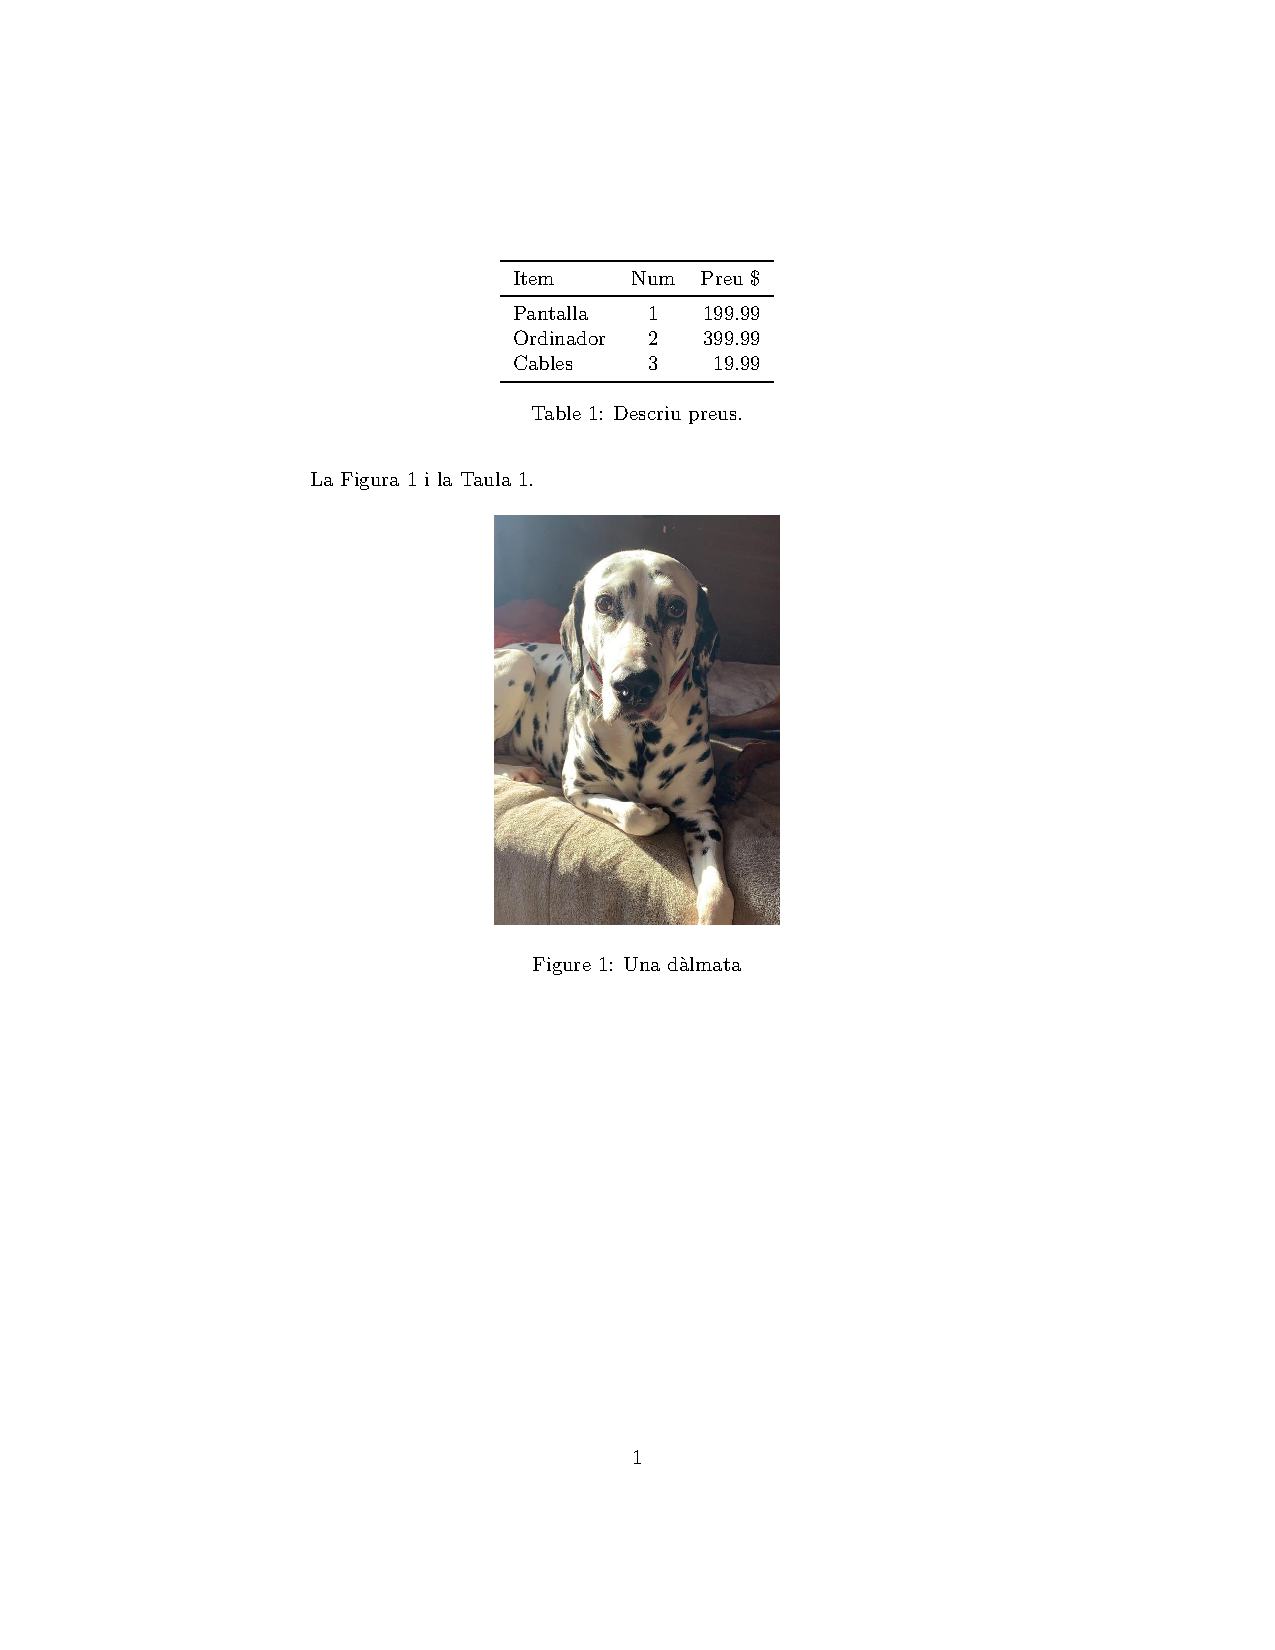
\includegraphics[width=\textwidth,clip,trim=2in 3in 3in 1in]{media-graphics-tables.pdf}
\end{minipage}
\end{frame}

%%%%%%%%%%%%%%%%%%%%%%%%%%%%%%%%%%%%%%%%%%%%%%%%%%%%%%%%%%%%%%%%%%%%%%%%%%%%%%%
%%%%%%%%%%%%%%%%%%%%%%%%%%%%%%%%%%%%%%%%%%%%%%%%%%%%%%%%%%%%%%%%%%%%%%%%%%%%%%%
%%%%%%%%%%%%%%%%%%%%%%%%%%%%%%%%%%%%%%%%%%%%%%%%%%%%%%%%%%%%%%%%%%%%%%%%%%%%%%%
\begin{frame}[fragile]{Repassem: Matemàtiques}
\begin{itemize}
\item Els símbols de dòlar \keystrokebftt{\$} marquen matemàtiques al text.
\begin{exampletwouptiny}
% meh:
Siguin a i b nombres enters 
positius, i sigui c > a - b + 1

% millor:
Siguin $a$ i $b$ nombres enters 
positius, i sigui $c > a - b + 1$.
\end{exampletwouptiny}
\item Utilitza sempre els símbols de dòlar amb parelles: un per començar les matemàtiques, i un per acabar-les.
\end{itemize}
\end{frame}

%%%%%%%%%%%%%%%%%%%%%%%%%%%%%%%%%%%%%%%%%%%%%%%%%%%%%%%%%%%%%%%%%%%%%%%%%%%%%%%
%%%%%%%%%%%%%%%%%%%%%%%%%%%%%%%%%%%%%%%%%%%%%%%%%%%%%%%%%%%%%%%%%%%%%%%%%%%%%%%
%%%%%%%%%%%%%%%%%%%%%%%%%%%%%%%%%%%%%%%%%%%%%%%%%%%%%%%%%%%%%%%%%%%%%%%%%%%%%%%
\begin{frame}[fragile]{Taules: més opcions}
Hi ha moltes opcions diferents per fer taules.
\begin{itemize}
\item Es poden fusionar columnes amb \cmdbs{multicolumn} i files amb \cmdbs{multirow} (cal el paquet \bftt{multirow}).
\item Línies horitzontals més curtes amb \cmdbs{cline} o \cmdbs{cmidrule} de \bftt{booktabs}.
\end{itemize}

\begin{exampletwouptiny}
\begin{tabular}{lrr}
\toprule
Item &
\multicolumn{2}{c}{MultiColumna} \\
\cline{2-3}
Pantalla                   & 1 & 2.99\\
\cmidrule{1-2}
\multirow{2}{*}{MultiFila} & 2 & 3.99\\
                           & 3 & 1.99\\
\bottomrule
\end{tabular}
\end{exampletwouptiny}
\end{frame}


%%%%%%%%%%%%%%%%%%%%%%%%%%%%%%%%%%%%%%%%%%%%%%%%%%%%%%%%%%%%%%%%%%%%%%%%%%%%%%%
%%%%%%%%%%%%%%%%%%%%%%%%%%%%%%%%%%%%%%%%%%%%%%%%%%%%%%%%%%%%%%%%%%%%%%%%%%%%%%%
%%%%%%%%%%%%%%%%%%%%%%%%%%%%%%%%%%%%%%%%%%%%%%%%%%%%%%%%%%%%%%%%%%%%%%%%%%%%%%%
\begin{frame}[fragile]{Repassem: Dubtes classe anterior}
\begin{itemize}
    \item \textbf{Com s'escapa una seqüència sencera?}\\
    Cal escapar la pròpia barra inversa \keystroke{\textbackslash} amb \cmd{\textbackslash{}textbackslash{}}.

\begin{exampletwouptiny}
% podem separar l'ordre amb espai
\textbackslash includegraphics

% o amb claus
\textbackslash{}includegraphics
\end{exampletwouptiny}
\item \textbf{Com s'evita que es tallin paraules amb guió a final de línia?}
Es pot posar el següent al preàmbul (\href{https://tex.stackexchange.com/questions/5036/how-to-prevent-latex-from-hyphenating-the-entire-document}{font}):

\begin{exampletiny}
\tolerance=1
\emergencystretch=\maxdimen
\hyphenpenalty=10000
\hbadness=10000
\end{exampletiny}
\end{itemize}
\end{frame}


%%%%%%%%%%%%%%%%%%%%%%%%%%%%%%%%%%%%%%%%%%%%%%%%%%%%%%%%%%%%%%%%%%%%%%%%%%%%%%%
%%%%%%%%%%%%%%%%%%%%%%%%%%%%%%%%%%%%%%%%%%%%%%%%%%%%%%%%%%%%%%%%%%%%%%%%%%%%%%%
%%%%%%%%%%%%%%%%%%%%%%%%%%%%%%%%%%%%%%%%%%%%%%%%%%%%%%%%%%%%%%%%%%%%%%%%%%%%%%%
\section{Estructura i format}
\begin{frame}{Continguts}
\begin{multicols}{2}
\tableofcontents[currentsection]
\end{multicols}
\end{frame}

%%%%%%%%%%%%%%%%%%%%%%%%%%%%%%%%%%%%%%%%%%%%%%%%%%%%%%%%%%%%%%%%%%%%%%%%%%%%%%%
%%%%%%%%%%%%%%%%%%%%%%%%%%%%%%%%%%%%%%%%%%%%%%%%%%%%%%%%%%%%%%%%%%%%%%%%%%%%%%%
%%%%%%%%%%%%%%%%%%%%%%%%%%%%%%%%%%%%%%%%%%%%%%%%%%%%%%%%%%%%%%%%%%%%%%%%%%%%%%%
\subsection{Títol i Resum}
\begin{frame}[fragile]{Títol i Resum}
\begin{itemize}{\small
\item A \LaTeX{}, \cmdbs{title}, \cmdbs{author} i \cmdbs{date}\footnote{Si no volem data ho deixem buit.} es defineixen al preàmbul.
\item Dins el document, \cmdbs{maketitle} crea el títol.
\item Utilitza l'entorn \bftt{abstract} per crear un resum.
\item El paquet \bftt{babel} defineix l'idioma del document.
}\end{itemize}
\begin{minipage}{0.55\linewidth}
\inputminted[fontsize=\scriptsize,frame=single,resetmargins]{latex}%
  {structure-title.tex}
\end{minipage}
\begin{minipage}{0.35\linewidth}
\includegraphics[width=1.3\textwidth,clip,trim=2.4in 7in 2.4in 2in]{structure-title.pdf}
\end{minipage}
\end{frame}

%%%%%%%%%%%%%%%%%%%%%%%%%%%%%%%%%%%%%%%%%%%%%%%%%%%%%%%%%%%%%%%%%%%%%%%%%%%%%%%
%%%%%%%%%%%%%%%%%%%%%%%%%%%%%%%%%%%%%%%%%%%%%%%%%%%%%%%%%%%%%%%%%%%%%%%%%%%%%%%
%%%%%%%%%%%%%%%%%%%%%%%%%%%%%%%%%%%%%%%%%%%%%%%%%%%%%%%%%%%%%%%%%%%%%%%%%%%%%%%
\subsection{Seccions}
\begin{frame}{Seccions}
\begin{itemize}{\small
    \item \cmdbs{section} i \cmdbs{subsection}
        (\href{https://www.overleaf.com/learn/latex/Sections_and_chapters}{hi ha més nivells})
\item Què creus que fan \cmdbs{section*} i \cmdbs{subsection*}?
}\end{itemize}
\begin{minipage}{0.55\linewidth}
\inputminted[fontsize=\scriptsize,frame=single,resetmargins]{latex}%
  {structure-sections.tex}
\end{minipage}
\begin{minipage}{0.35\linewidth}
\includegraphics[width=\textwidth,clip,trim=1.5in 6in 4in 1in]{structure-sections.pdf}
\end{minipage}
\end{frame}

%%%%%%%%%%%%%%%%%%%%%%%%%%%%%%%%%%%%%%%%%%%%%%%%%%%%%%%%%%%%%%%%%%%%%%%%%%%%%%%
%%%%%%%%%%%%%%%%%%%%%%%%%%%%%%%%%%%%%%%%%%%%%%%%%%%%%%%%%%%%%%%%%%%%%%%%%%%%%%%
%%%%%%%%%%%%%%%%%%%%%%%%%%%%%%%%%%%%%%%%%%%%%%%%%%%%%%%%%%%%%%%%%%%%%%%%%%%%%%%
\begin{frame}{Índexs}
\begin{itemize}{\small
    \item \cmdbs{tableofcontents} crea l'índex general.
    \item \cmdbs{listoffigures} i \cmdbs{listoftables} creen l'índex de figures i de taules.
    \item \LaTeX{} també facilita la creació d'\href{https://www.overleaf.com/learn/latex/Indices}{índexs analítics}.
}\end{itemize}
%Com els podem canviar el nom? 
\begin{minipage}{0.55\linewidth}
\inputminted[fontsize=\scriptsize,frame=single,resetmargins]{latex}%
  {structure-sections-toc.tex}
\end{minipage}
\begin{minipage}{0.35\linewidth}
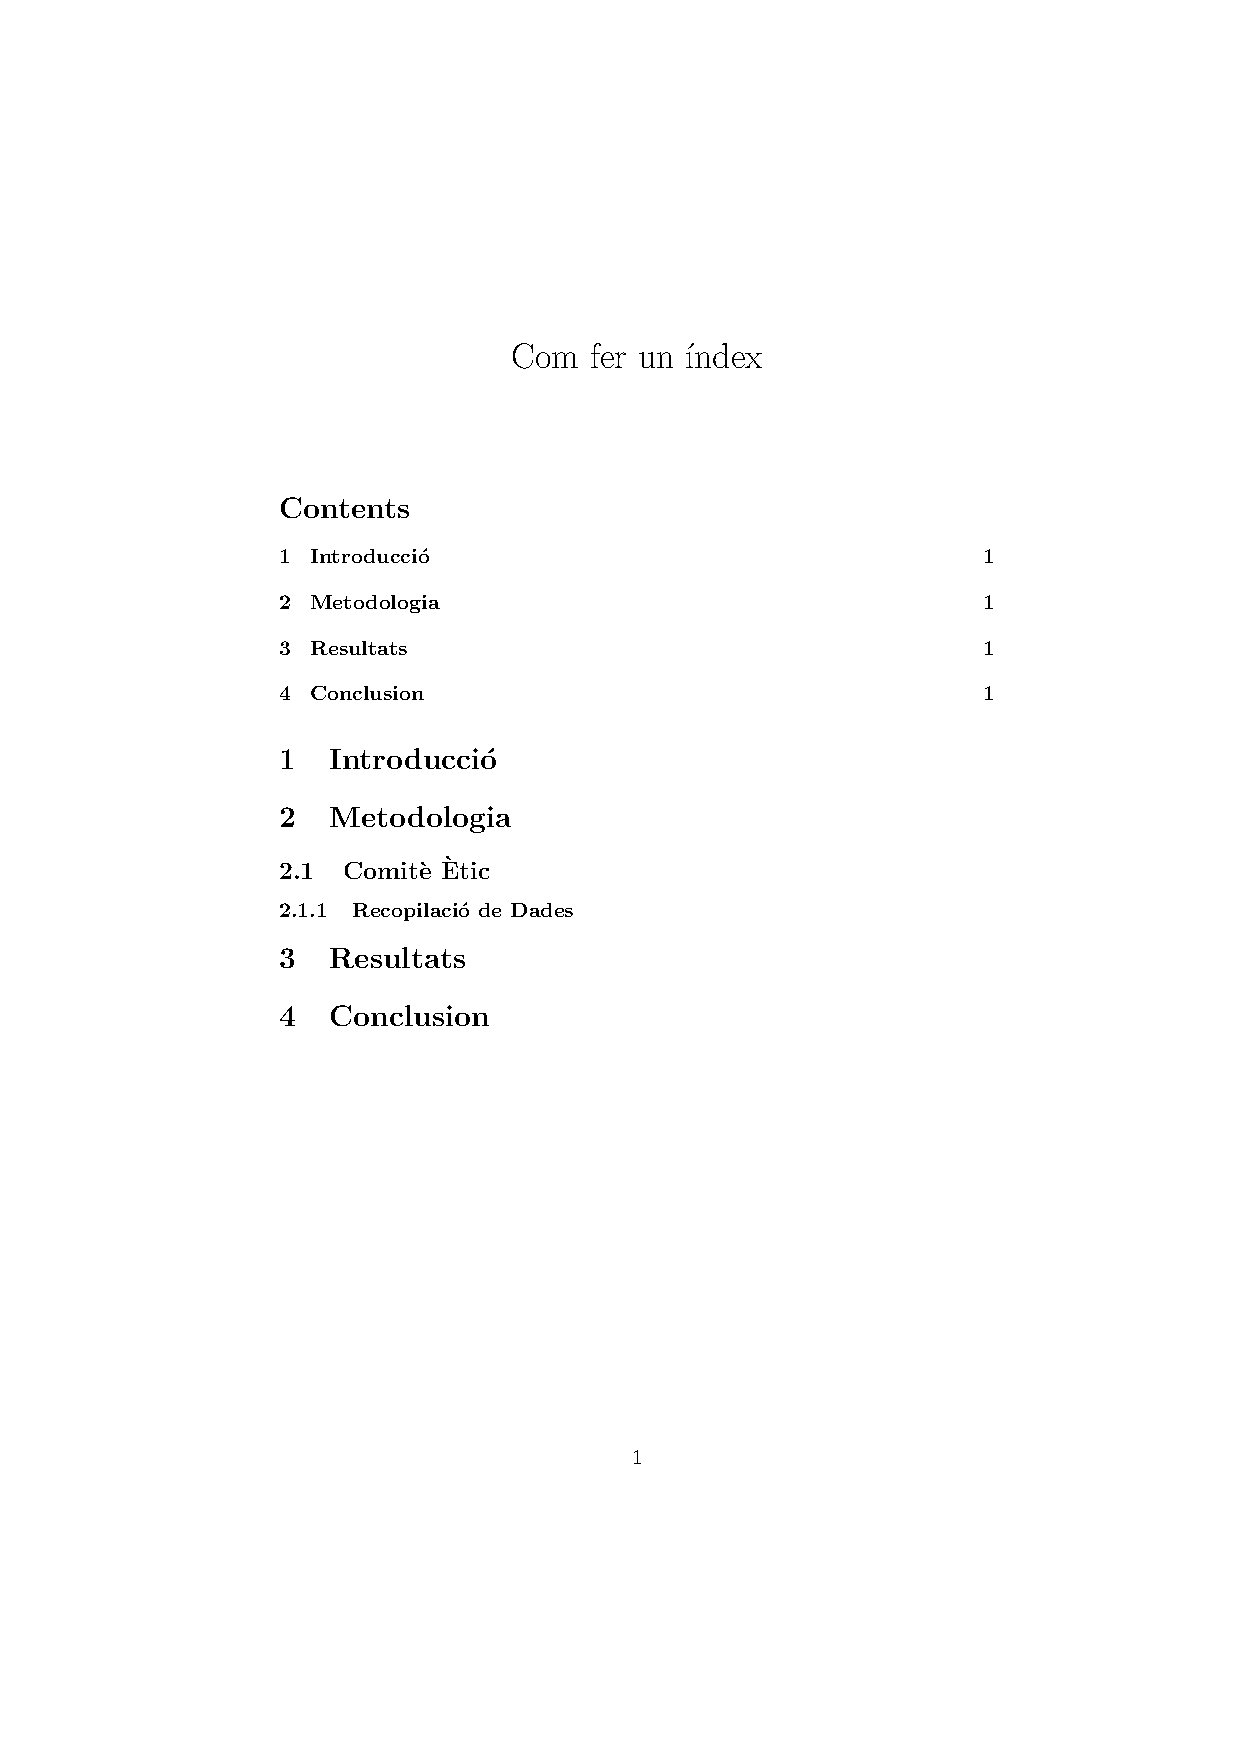
\includegraphics[width=\textwidth,clip,trim=1.5in 4in 1.5in 2in]{structure-sections-toc.pdf}
\end{minipage}
\end{frame}


%%%%%%%%%%%%%%%%%%%%%%%%%%%%%%%%%%%%%%%%%%%%%%%%%%%%%%%%%%%%%%%%%%%%%%%%%%%%%%%
%%%%%%%%%%%%%%%%%%%%%%%%%%%%%%%%%%%%%%%%%%%%%%%%%%%%%%%%%%%%%%%%%%%%%%%%%%%%%%%
%%%%%%%%%%%%%%%%%%%%%%%%%%%%%%%%%%%%%%%%%%%%%%%%%%%%%%%%%%%%%%%%%%%%%%%%%%%%%%%
\begin{frame}[fragile]{Format: marges i interlineat}
\begin{itemize}
\item El paquet \bftt{geometry} ens permet modificar la \href{https://www.overleaf.com/learn/latex/Page_size_and_margins}{mida i els marges del document}.
\item \bftt{setspace} defineix l'interlineat amb les ordres \cmdbs{singlespacing}, \cmdbs{onehalfspacing}, \cmdbs{doublespacing}\footnote{No hi ha una definició clara de què vol dir interlineat doble.}, o un valor personalitzat amb \cmdbs{setstretch}. Més informació sobre espaiat \href{https://www.overleaf.com/learn/latex/Articles/How_to_change_paragraph_spacing_in_LaTeX#The_setspace_package}{aquí}.
\end{itemize}

\begin{exampletiny}
\usepackage{geometry}
\geometry{
a4paper,
left=30mm,
right=30mm,
top=25mm,
bottom=25mm,
}

\usepackage{setspace}
\setstretch{1.6}  
\end{exampletiny}

\end{frame}

%%%%%%%%%%%%%%%%%%%%%%%%%%%%%%%%%%%%%%%%%%%%%%%%%%%%%%%%%%%%%%%%%%%%%%%%%%%%%%%
%%%%%%%%%%%%%%%%%%%%%%%%%%%%%%%%%%%%%%%%%%%%%%%%%%%%%%%%%%%%%%%%%%%%%%%%%%%%%%%
%%%%%%%%%%%%%%%%%%%%%%%%%%%%%%%%%%%%%%%%%%%%%%%%%%%%%%%%%%%%%%%%%%%%%%%%%%%%%%%
\subsection{Etiquetes i Referències Creuades}
\begin{frame}[fragile]{Etiquetes i Referències Creuades}
\begin{itemize}{\small
\item \cmdbs{label} serveix per etiquetar i \cmdbs{ref} per referenciar.
\item Les dues serveixen per seccions, figures, taules \dots
}\end{itemize}
\begin{minipage}{0.60\linewidth}
\inputminted[fontsize=\scriptsize,frame=single,resetmargins]{latex}%
  {structure-crossref.tex}
\end{minipage}
\begin{minipage}{0.3\linewidth}
\includegraphics[width=\textwidth,clip,trim=1.5in 6in 4in 1in]{structure-crossref.pdf}
\end{minipage}
\end{frame}

%%%%%%%%%%%%%%%%%%%%%%%%%%%%%%%%%%%%%%%%%%%%%%%%%%%%%%%%%%%%%%%%%%%%%%%%%%%%%%%
%%%%%%%%%%%%%%%%%%%%%%%%%%%%%%%%%%%%%%%%%%%%%%%%%%%%%%%%%%%%%%%%%%%%%%%%%%%%%%%
%%%%%%%%%%%%%%%%%%%%%%%%%%%%%%%%%%%%%%%%%%%%%%%%%%%%%%%%%%%%%%%%%%%%%%%%%%%%%%%
\begin{frame}[fragile]{Etiquetes i Referències Creuades: hyperref}
\begin{itemize}{\small
\item El paquet \bftt{hyperref} converteix totes les referències creuades en ``hyperlinks''. Només cal afegir-lo amb \cmdbs{usepackage}.
\item Podem canviar l'aparença de les referències. Per exemple, per aquesta presentació:
\begin{exampletiny}
\usepackage{hyperref}
\hypersetup{colorlinks,breaklinks,urlcolor=magenta,linkcolor=black}
\end{exampletiny}
\item Si voleu mantenir els enllaços, però sense cap color, feu servir:
\begin{exampletiny}
\hypersetup{hidelinks=true}
\end{exampletiny}

\item També defineix les ordres \cmdbs{url}\footnote{Si només voleu una URL també existeix el paquet \bftt{url}.}
    i \cmdbs{href} per referir-se a pàgines web.
}\end{itemize}
\begin{exampletiny}
\url{https://www.overleaf.com/learn/latex/Hyperlinks}

\href{https://www.overleaf.com/learn/latex/Hyperlinks}{Exemple}
\end{exampletiny}

\url{https://www.overleaf.com/learn/latex/Hyperlinks}

\href{https://www.overleaf.com/learn/latex/Hyperlinks}{Exemple}
\end{frame}

%%%%%%%%%%%%%%%%%%%%%%%%%%%%%%%%%%%%%%%%%%%%%%%%%%%%%%%%%%%%%%%%%%%%%%%%%%%%%%%
%%%%%%%%%%%%%%%%%%%%%%%%%%%%%%%%%%%%%%%%%%%%%%%%%%%%%%%%%%%%%%%%%%%%%%%%%%%%%%%
%%%%%%%%%%%%%%%%%%%%%%%%%%%%%%%%%%%%%%%%%%%%%%%%%%%%%%%%%%%%%%%%%%%%%%%%%%%%%%%
% \begin{frame}[fragile]{\protect\bftt{cleveref}: Millors Referències Creuades (opinió)}
% \begin{itemize}{\small
% \item \bftt{cleveref} permet tenir automàticament el nom del que estiguem referenciant.
% \item Només cal canviar \cmdbs{ref} per \cmdbs{cref}, i serveix per seccions, figures i taules.
% }\end{itemize}
% \begin{minipage}{0.55\linewidth}
% \inputminted[fontsize=\scriptsize,frame=single,resetmargins]{latex}%
%   {structure-cleveref.tex}
% \end{minipage}
% \begin{minipage}{0.35\linewidth}
% 
\includegraphics[width=\textwidth,clip,trim=1.5in 6in 4in 1in]{structure-cleveref.pdf}
% \end{minipage}
% \end{frame}

%%%%%%%%%%%%%%%%%%%%%%%%%%%%%%%%%%%%%%%%%%%%%%%%%%%%%%%%%%%%%%%%%%%%%%%%%%%%%%%
%%%%%%%%%%%%%%%%%%%%%%%%%%%%%%%%%%%%%%%%%%%%%%%%%%%%%%%%%%%%%%%%%%%%%%%%%%%%%%%
%%%%%%%%%%%%%%%%%%%%%%%%%%%%%%%%%%%%%%%%%%%%%%%%%%%%%%%%%%%%%%%%%%%%%%%%%%%%%%%
\subsection{Exercici}
\begin{frame}[fragile]{Exercici Document Estructurat}

\begin{block}{Escriu el següent article amb \LaTeX
\footnote{De \url{http://pdos.csail.mit.edu/scigen/},
un generador d'articles aleatoris.}:}
\begin{center}
\fbox{\href{\fileuri/structure-exercise-solution.pdf}{Clica per obrir l'article}}
\end{center}
Fes servir interlineat doble, marges de 2 cm als laterals, i de 1,5cm a dalt i a baix.
Utilitza \cmdbs{ref} per evitar escriure explícitament el número de les seccions.
Posa el paquet \bftt{hyperref} al preàmbul.
\end{block}
\vskip 2ex
\begin{center}
\fbox{\href{\wlnewdoc{structure-exercise.tex}}{%
Clica per obrir l'exercici a \wllogo{}}}
\end{center}

\begin{itemize}
\item Un cop ho hagis provat,
\fbox{\href{\wlnewdoc{structure-exercise-solution.tex}}{%
Clica per veure la solució}}.
\end{itemize}
\end{frame}

%%%%%%%%%%%%%%%%%%%%%%%%%%%%%%%%%%%%%%%%%%%%%%%%%%%%%%%%%%%%%%%%%%%%%%%%%%%%%%%
%%%%%%%%%%%%%%%%%%%%%%%%%%%%%%%%%%%%%%%%%%%%%%%%%%%%%%%%%%%%%%%%%%%%%%%%%%%%%%%
%%%%%%%%%%%%%%%%%%%%%%%%%%%%%%%%%%%%%%%%%%%%%%%%%%%%%%%%%%%%%%%%%%%%%%%%%%%%%%%
\subsection{Format}
\begin{frame}[fragile]{Format: tipus de document}
\begin{itemize}
\item A part d'\textbf{article} les classes més típiques són \textbf{report} (llibres curts o tesis), \textbf{book} i \textbf{beamer} (diapositives).
\item Tot i això, hi ha \href{https://ctan.org/topic/class}{una multitud de classes}, bàsicament pensades per revistes concretes, com \textbf{apa} o \textbf{amsart}.
\item Famílies de paquets com \href{https://ctan.org/pkg/koma-script}{KOMA-Script} tenen moltes opcions, amb equivalents per article (\textbf{scrartcl}), report (\textbf{scrreprt}) i book (\textbf{scrbook}). Si les voleu utilitzar carregueu també el paquet \bftt{lmodern}. Una altra família és \href{https://ctan.org/pkg/minimalist}{minimalist} (conté l'estil \textbf{ClassicThesis})
\item \href{https://ctan.org/pkg/memoir}{memoir} s'utilitza per escriure llibres professionalment.
\end{itemize}

\begin{exampletiny}
\documentclass{scrartcl}
\usepackage{lmodern}
\end{exampletiny}

\end{frame}


%%%%%%%%%%%%%%%%%%%%%%%%%%%%%%%%%%%%%%%%%%%%%%%%%%%%%%%%%%%%%%%%%%%%%%%%%%%%%%%
%%%%%%%%%%%%%%%%%%%%%%%%%%%%%%%%%%%%%%%%%%%%%%%%%%%%%%%%%%%%%%%%%%%%%%%%%%%%%%%
%%%%%%%%%%%%%%%%%%%%%%%%%%%%%%%%%%%%%%%%%%%%%%%%%%%%%%%%%%%%%%%%%%%%%%%%%%%%%%%
\begin{frame}[fragile]{Format: negreta, cursiva, subratllat \dots}
\small{Ja hem vist que la negreta es fa amb \cmdbs{textbf} i la cursiva amb \cmdbs{textit}. \\
Què més es pot fer? \\
-- Canviar \href{https://www.overleaf.com/learn/latex/Font_sizes%2C_families%2C_and_styles}{la mida}
    o \href{https://www.overleaf.com/learn/latex/Using_colors_in_LaTeX}{el color} (paquet \bftt{xcolor})
}
\begin{exampletwouptiny2}
\textsc{Versaletes (Small Caps)}

\underline{subrallat}

\tiny{text}
\scriptsize{text}
\footnotesize{text}
\small{text}
\normalsize{text}
\large{text}
\Large{text}
\LARGE{text}
\huge{text}
\end{exampletwouptiny2}
\begin{exampletwouptiny2}
\begin{itemize}
\color{blue}
\item primer 
\item segon
\end{itemize}

\textcolor{red}{Text en vermell}
\colorbox{orange}{o amb color de fons}

\textcolor{cyan}{\underline{\large{
    \textit{\textbf{Tot junt}}}}}
\end{exampletwouptiny2}

\end{frame}


%%%%%%%%%%%%%%%%%%%%%%%%%%%%%%%%%%%%%%%%%%%%%%%%%%%%%%%%%%%%%%%%%%%%%%%%%%%%%%%
%%%%%%%%%%%%%%%%%%%%%%%%%%%%%%%%%%%%%%%%%%%%%%%%%%%%%%%%%%%%%%%%%%%%%%%%%%%%%%%
%%%%%%%%%%%%%%%%%%%%%%%%%%%%%%%%%%%%%%%%%%%%%%%%%%%%%%%%%%%%%%%%%%%%%%%%%%%%%%%
\section{Bibliografies}
\begin{frame}{Continguts}
\begin{multicols}{2}
\tableofcontents[currentsection]
\end{multicols}
\end{frame}

%%%%%%%%%%%%%%%%%%%%%%%%%%%%%%%%%%%%%%%%%%%%%%%%%%%%%%%%%%%%%%%%%%%%%%%%%%%%%%%
%%%%%%%%%%%%%%%%%%%%%%%%%%%%%%%%%%%%%%%%%%%%%%%%%%%%%%%%%%%%%%%%%%%%%%%%%%%%%%%
%%%%%%%%%%%%%%%%%%%%%%%%%%%%%%%%%%%%%%%%%%%%%%%%%%%%%%%%%%%%%%%%%%%%%%%%%%%%%%%
\subsection{Bib\LaTeX{}}
\begin{frame}[fragile]{Bib\LaTeX{} 1}
\begin{itemize}
\item Poseu les referències a un fitxer \bftt{.bib} en format `bibtex':
\vskip 1ex
\inputminted[fontsize=\scriptsize,frame=single]{latex}{bib-example.bib}
\item La majoria de gestors i buscadors d'articles ofereixen aquesta opció.
\end{itemize}
\end{frame}

%%%%%%%%%%%%%%%%%%%%%%%%%%%%%%%%%%%%%%%%%%%%%%%%%%%%%%%%%%%%%%%%%%%%%%%%%%%%%%%
%%%%%%%%%%%%%%%%%%%%%%%%%%%%%%%%%%%%%%%%%%%%%%%%%%%%%%%%%%%%%%%%%%%%%%%%%%%%%%%
%%%%%%%%%%%%%%%%%%%%%%%%%%%%%%%%%%%%%%%%%%%%%%%%%%%%%%%%%%%%%%%%%%%%%%%%%%%%%%%
\begin{frame}[fragile]{Bib\LaTeX{} 2}
\begin{itemize}
\item Cada entrada del fitxer \bftt{.bib} té una clau que serveix per referenciar-la dins el text.
Per exemple, \bftt{Jacobson1999Towards} és la clau d'aquest article:
\begin{minted}[fontsize=\small,frame=single]{latex}
@Article{Jacobson1999Towards,
  author = {Van Jacobson},
  ...
}
\end{minted}
\item És bona idea canviar la clau que trobeu per defecte a una que contingui nom any i títol.
\item \LaTeX{} formatejarà automàticament les cites en el format adequat (Science, APA, Chicago \dots), tant dins al text com a l'apartat de referències.
\end{itemize}
\end{frame}

%%%%%%%%%%%%%%%%%%%%%%%%%%%%%%%%%%%%%%%%%%%%%%%%%%%%%%%%%%%%%%%%%%%%%%%%%%%%%%%
%%%%%%%%%%%%%%%%%%%%%%%%%%%%%%%%%%%%%%%%%%%%%%%%%%%%%%%%%%%%%%%%%%%%%%%%%%%%%%%
%%%%%%%%%%%%%%%%%%%%%%%%%%%%%%%%%%%%%%%%%%%%%%%%%%%%%%%%%%%%%%%%%%%%%%%%%%%%%%%
\begin{frame}[fragile]{Bib\LaTeX{} 3}
\begin{itemize}\small{
\item Feu servir el paquet \bftt{biblatex}\footnote{Hi ha un altre paquet (més vell) de referència, \bftt{natbib}. És possible que us el trobeu a alguna plantilla. Fa servir \cmdbs{citet} i \cmdbs{citep}.}
    amb \cmdbs{cite} (genèric), \cmdbs{citetext} (textual) i \cmdbs{parencite} (entre parèntesis).
\item Al final del document poseu \cmdbs{printbibliography}
}\end{itemize}
\begin{minipage}{0.45\linewidth}
\inputminted[fontsize=\tiny,frame=single,resetmargins]{latex}%
  {bib-example.tex}
\end{minipage}
\begin{minipage}{0.4\linewidth}
\includegraphics[width=1.4\textwidth,clip,trim=1.8in 5in 1.6in 1in]{bib-example.pdf}
\end{minipage}
\end{frame}

%%%%%%%%%%%%%%%%%%%%%%%%%%%%%%%%%%%%%%%%%%%%%%%%%%%%%%%%%%%%%%%%%%%%%%%%%%%%%%%
%%%%%%%%%%%%%%%%%%%%%%%%%%%%%%%%%%%%%%%%%%%%%%%%%%%%%%%%%%%%%%%%%%%%%%%%%%%%%%%
%%%%%%%%%%%%%%%%%%%%%%%%%%%%%%%%%%%%%%%%%%%%%%%%%%%%%%%%%%%%%%%%%%%%%%%%%%%%%%%
\subsection{Exercici}
\begin{frame}[fragile]{Exercici: Pose-m'ho tot junt}

Afegiu una imatge (referenciada al text) i bibliografia a l'article de l'exercici anterior.
Feu almenys una cita textual i una de parentètica.

\begin{enumerate}
\item Baixeu-vos aquests fitxers d'exemple (o els vostres propis).

\begin{center}
\fbox{\href{\fileuri/figures/gus_gran.png?dl=1}{Clica per baixar la imatge d'exemple}}

\fbox{\href{\fileuri/bib-exercise.bib?dl=1}{Clica per descarregar fitxer BIB d'exemple}}
\end{center}

\item Pujeu-los a Overleaf.

\end{enumerate}
\end{frame}

%%%%%%%%%%%%%%%%%%%%%%%%%%%%%%%%%%%%%%%%%%%%%%%%%%%%%%%%%%%%%%%%%%%%%%%%%%%%%%%
%%%%%%%%%%%%%%%%%%%%%%%%%%%%%%%%%%%%%%%%%%%%%%%%%%%%%%%%%%%%%%%%%%%%%%%%%%%%%%%
%%%%%%%%%%%%%%%%%%%%%%%%%%%%%%%%%%%%%%%%%%%%%%%%%%%%%%%%%%%%%%%%%%%%%%%%%%%%%%%
\section{Exemples lingüístics}
\begin{frame}{Continguts}
\begin{multicols}{2}
\tableofcontents[currentsection]
\end{multicols}
\end{frame}


%%%%%%%%%%%%%%%%%%%%%%%%%%%%%%%%%%%%%%%%%%%%%%%%%%%%%%%%%%%%%%%%%%%%%%%%%%%%%%%
%%%%%%%%%%%%%%%%%%%%%%%%%%%%%%%%%%%%%%%%%%%%%%%%%%%%%%%%%%%%%%%%%%%%%%%%%%%%%%%
%%%%%%%%%%%%%%%%%%%%%%%%%%%%%%%%%%%%%%%%%%%%%%%%%%%%%%%%%%%%%%%%%%%%%%%%%%%%%%%
\subsection{linguex}
\begin{frame}[fragile]{linguex: exemples}
\begin{itemize}
\item Les 3 ordres bàsiques de linguex són \cmdbs{ex.}, \cmdbs{a.} i \cmdbs{b.}.
\item \cmdbs{ex.} inicia l'exemple, i \textbf{cal una línia en blanc} per acabar-lo.
\begin{exampletwouptiny2}
\ex. Exemple

\ex. Primer nivell de l'exemple
\a. Segon nivell de l'exemple
\b. Seguim al segon nivell

\ex.
\a. podem deixar buit
\b. el primer nivell
\c. si volem ser ordenats
\d. podem fer servir
\e. tot l'abecedari
\b. tot i que no cal

\end{exampletwouptiny2}
\item Les ordres \cmdbs{c.}, \cmdbs{d.}, etc.~són còpies de \cmdbs{b.}.
\item \bftt{linguex} és senzill, però, tot i poder-se modificar, és limitat. Hi ha paquets més potents però amb una sintaxi més complexa. \href{https://www.jostellings.com/numbex.html}{Vegeu aquesta breu explicació}. 
\end{itemize}
\end{frame}

%%%%%%%%%%%%%%%%%%%%%%%%%%%%%%%%%%%%%%%%%%%%%%%%%%%%%%%%%%%%%%%%%%%%%%%%%%%%%%%
%%%%%%%%%%%%%%%%%%%%%%%%%%%%%%%%%%%%%%%%%%%%%%%%%%%%%%%%%%%%%%%%%%%%%%%%%%%%%%%
%%%%%%%%%%%%%%%%%%%%%%%%%%%%%%%%%%%%%%%%%%%%%%%%%%%%%%%%%%%%%%%%%%%%%%%%%%%%%%%
\begin{frame}[fragile]{linguex: referències}
\begin{itemize}
\item Podem fer servir \cmdbs{label} i \cmdbs{ref}.
\item També podem referir-nos als exemples més propers amb \cmdbs{Next}, \cmdbs{Last}, \cmdbs{NNext} i \cmdbs{LLast}, fins i tot si no tenen una etiqueta.
\end{itemize}
\begin{exampletwouptiny2}
A l'exemple \ref{ex:1} hi ha faltes. 
\ex. Ejenple
\label{ex:1}

\ex. Primer nivell de l'exemple
\a. Segon nivell de l'exemple

Com hem vist a \LLast i \Last \dots

En canvi a \Next i \NNext veiem \dots

\ex.
\a. podem deixar buit
\b. el primer nivell

\ex. 
\label{ex:2}
\a. podem citar subexemples 
\label{ex:2a}
\b. posant label a sota 
\label{ex:2b}

Exemple \ref{ex:2} amb subexemples 
\ref{ex:2a} i \ref{ex:2b}.

\end{exampletwouptiny2}
\end{frame}

%%%%%%%%%%%%%%%%%%%%%%%%%%%%%%%%%%%%%%%%%%%%%%%%%%%%%%%%%%%%%%%%%%%%%%%%%%%%%%%
%%%%%%%%%%%%%%%%%%%%%%%%%%%%%%%%%%%%%%%%%%%%%%%%%%%%%%%%%%%%%%%%%%%%%%%%%%%%%%%
%%%%%%%%%%%%%%%%%%%%%%%%%%%%%%%%%%%%%%%%%%%%%%%%%%%%%%%%%%%%%%%%%%%%%%%%%%%%%%%
\begin{frame}[fragile]{linguex: exemples 2}
\begin{itemize}
\item Per acabar un sol nivell s'utilitza \cmdbs{z.}
\begin{exampletwouptiny2}
\ex. Animals
\a. Gats
\a. miau
\z.
\b. Gossos
\a. bup
\z.
\b. Fures

\end{exampletwouptiny2}
\end{itemize}

\end{frame}

%%%%%%%%%%%%%%%%%%%%%%%%%%%%%%%%%%%%%%%%%%%%%%%%%%%%%%%%%%%%%%%%%%%%%%%%%%%%%%%
%%%%%%%%%%%%%%%%%%%%%%%%%%%%%%%%%%%%%%%%%%%%%%%%%%%%%%%%%%%%%%%%%%%%%%%%%%%%%%%
%%%%%%%%%%%%%%%%%%%%%%%%%%%%%%%%%%%%%%%%%%%%%%%%%%%%%%%%%%%%%%%%%%%%%%%%%%%%%%%
\begin{frame}[fragile]{linguex: gramaticalitat}
\begin{itemize}
    \item Linguex admet els símbols *, ?, \# i \% per judicis de gramaticalitat (els posa al davant)\footnote{recordeu que \# i \% s'escriuen amb una \keystroke{\textbackslash} davant}.
\begin{exampletwouptiny2}
\ex.
\a. Exemple ben format
\b. * Agramatical frase?
\b. ** i molt agramatical molt
\b. \# El formatge l'hi he posat
\c. ? Hi han maduixes

\end{exampletwouptiny2}
\end{itemize}

\end{frame}

%%%%%%%%%%%%%%%%%%%%%%%%%%%%%%%%%%%%%%%%%%%%%%%%%%%%%%%%%%%%%%%%%%%%%%%%%%%%%%%
%%%%%%%%%%%%%%%%%%%%%%%%%%%%%%%%%%%%%%%%%%%%%%%%%%%%%%%%%%%%%%%%%%%%%%%%%%%%%%%
%%%%%%%%%%%%%%%%%%%%%%%%%%%%%%%%%%%%%%%%%%%%%%%%%%%%%%%%%%%%%%%%%%%%%%%%%%%%%%%
\begin{frame}[fragile]{linguex: glosses}
\begin{itemize}
\item Linguex és molt últil per morfologia.
\item Per glossar un exemple afegim `g' després de l'última lletra de l'ordre i linguex s'encarrega d'alinear les paraules (cal \keystrokebftt{\bs\bs}  per marcar el final de línia).
\begin{exampletwouptiny2}
\ex.\a. No gloss
\bg. This is a first gloss\\
Dies ist eine erste Glosse\\

\exg.
Dies ist nicht die erste Glosse\\
This is not the first gloss\\

\end{exampletwouptiny2}
\item Podem afegir una tercera línia de traducció amb \cmdbs{glt} (gloss translation).
\begin{exampletwouptiny2}
\exg.
Martin-ek Diego-\zero{} ikusi du \\
Martin-ERG Diego-ABS vist ha \\
\glt `En Martin ha vist en Diego'

\end{exampletwouptiny2}
\end{itemize}

\end{frame}

%%%%%%%%%%%%%%%%%%%%%%%%%%%%%%%%%%%%%%%%%%%%%%%%%%%%%%%%%%%%%%%%%%%%%%%%%%%%%%%
%%%%%%%%%%%%%%%%%%%%%%%%%%%%%%%%%%%%%%%%%%%%%%%%%%%%%%%%%%%%%%%%%%%%%%%%%%%%%%%
%%%%%%%%%%%%%%%%%%%%%%%%%%%%%%%%%%%%%%%%%%%%%%%%%%%%%%%%%%%%%%%%%%%%%%%%%%%%%%%
\begin{frame}[fragile]{linguex: glosses 2}
\begin{itemize}
\item Podem modificar les glosses perquè tinguin l'aspecte que vulguem.
\begin{exampletwouptiny}
\renewcommand{\eachwordone}{\itshape}
\renewcommand{\eachwordtwo}{\tiny}

\exg.
Martin-ek Diego-\zero{} ikusi du \\
Martin-ERG Diego-ABS vist ha \\
\glt `En Martin ha vist en Diego'


\end{exampletwouptiny}
\end{itemize}

\end{frame}

%%%%%%%%%%%%%%%%%%%%%%%%%%%%%%%%%%%%%%%%%%%%%%%%%%%%%%%%%%%%%%%%%%%%%%%%%%%%%%%
%%%%%%%%%%%%%%%%%%%%%%%%%%%%%%%%%%%%%%%%%%%%%%%%%%%%%%%%%%%%%%%%%%%%%%%%%%%%%%%
%%%%%%%%%%%%%%%%%%%%%%%%%%%%%%%%%%%%%%%%%%%%%%%%%%%%%%%%%%%%%%%%%%%%%%%%%%%%%%%
\begin{frame}[fragile]{linguex: claudators}
\begin{itemize}
\item Amb l'ordre \cmdbs{exi.} es pot fer servir notació amb claudators
\item Si l'exemple conté una glossa, cal saltar-se elements amb `\{\}'
\begin{MyMinted}
\exi.
\a.  [SC that [ST John$_i$  [Sv $t_i$ likes Mary ]]]
\bg. [SC dass [ST Peter$_i$ [Sv $t_i$ Mari liebt ]]] \\
{} that {} Peter {} {} Mary loves \\
\glt `that Peter loves Mary'
\end{MyMinted}
\exi.
\a.  [SC that [ST John$_i$  [Sv $t_i$ likes Mary ]]]
\bg. [SC dass [ST Peter$_i$ [Sv $t_i$ Mari liebt ]]] \\
{} that {} Peter {} {} Mary loves \\
\glt `that Peter loves Mary'

\end{itemize}

\end{frame}

%%%%%%%%%%%%%%%%%%%%%%%%%%%%%%%%%%%%%%%%%%%%%%%%%%%%%%%%%%%%%%%%%%%%%%%%%%%%%%%
%%%%%%%%%%%%%%%%%%%%%%%%%%%%%%%%%%%%%%%%%%%%%%%%%%%%%%%%%%%%%%%%%%%%%%%%%%%%%%%
%%%%%%%%%%%%%%%%%%%%%%%%%%%%%%%%%%%%%%%%%%%%%%%%%%%%%%%%%%%%%%%%%%%%%%%%%%%%%%%
\begin{frame}[fragile]{Extra: arbres}
\begin{itemize}
\item Hi ha dos paquets importants per fer arbres: \bftt{forest} i \bftt{tikz-qtree}.
\item Mireu els manuals per saber quin uns convé.
\begin{exampletwouptiny}
\ex. \begin{forest}
[SC[C][ST[T][SV[V][SN]]]]
\end{forest}

\end{exampletwouptiny}
\item \href{https://ling.auf.net/lingbuzz/003391}{Guia forest}
\end{itemize}

\end{frame}


%%%%%%%%%%%%%%%%%%%%%%%%%%%%%%%%%%%%%%%%%%%%%%%%%%%%%%%%%%%%%%%%%%%%%%%%%%%%%%%
%%%%%%%%%%%%%%%%%%%%%%%%%%%%%%%%%%%%%%%%%%%%%%%%%%%%%%%%%%%%%%%%%%%%%%%%%%%%%%%
%%%%%%%%%%%%%%%%%%%%%%%%%%%%%%%%%%%%%%%%%%%%%%%%%%%%%%%%%%%%%%%%%%%%%%%%%%%%%%%
\subsection{Exemple comentat}
\begin{frame}{Exemple comentat}
\href{https://www.overleaf.com/read/sxkcdfrpmbcb\#10abd3}{Treball morfologia basca} --- conté:
\begin{itemize}
    \item Un treball estructurat amb diversos fitxers, glosses personalitzades, taules amb format avançat i exemples de bibliografia tant amb biblatex com amb apacite.
    \item Una presentació amb \bftt{beamer} (ho veurem el següent dia).
\end{itemize}

\end{frame}

%%%%%%%%%%%%%%%%%%%%%%%%%%%%%%%%%%%%%%%%%%%%%%%%%%%%%%%%%%%%%%%%%%%%%%%%%%%%%%%
%%%%%%%%%%%%%%%%%%%%%%%%%%%%%%%%%%%%%%%%%%%%%%%%%%%%%%%%%%%%%%%%%%%%%%%%%%%%%%%
%%%%%%%%%%%%%%%%%%%%%%%%%%%%%%%%%%%%%%%%%%%%%%%%%%%%%%%%%%%%%%%%%%%%%%%%%%%%%%%

\begin{frame}{Referències en línia}
\begin{itemize}
\item \href{https://www.overleaf.com/learn}{The Overleaf Learn Wiki} --- tutorials i material de referència.
\item \href{http://en.wikibooks.org/wiki/LaTeX}{The \LaTeX{} Wikibook} --- més tutorials i material de referència.
\item \href{http://tex.stackexchange.com/}{\TeX{} Stack Exchange} --- preguntes i respostes
\item \href{http://www.latex-community.org/}{\LaTeX{} Community} --- fòrum
\item \href{http://ctan.org/}{Comprehensive \TeX{} Archive Network (CTAN)} --- documentació de paquets.
\item Qualsevol buscador us portarà a alguna d'aquestes pàgines.
\end{itemize}

Repositori del curs: \href{https://github.com/Pastells/curs-latex}{Pastells/curs-latex}

\end{frame}




%%%%%%%%%%%%%%%%%%%%%%%%%%%%%%%%%%%%%%%%%%%%%%%%%%%%%%%%%%%%%%%%%%%%%%%%%%%%%%%
%%%%%%%%%%%%%%%%%%%%%%%%%%%%%%%%%%%%%%%%%%%%%%%%%%%%%%%%%%%%%%%%%%%%%%%%%%%%%%%
%%%%%%%%%%%%%%%%%%%%%%%%%%%%%%%%%%%%%%%%%%%%%%%%%%%%%%%%%%%%%%%%%%%%%%%%%%%%%%%

\end{document}

\subsection{Tipografia}
\begin{frame}{Tipografia}
\begin{tabular}{lll}
& nom del símbol & s'usa per \dots \\\hline
\bftt{\bs} & backslash                 & ordres, tables \\
\bftt{\{}  & open brace                & ordres \\
\bftt{\}}  & close brace               & ordres \\
\bftt{\%}  & percent sign              & comments \\
\bftt{\#}  & hash (pound / sharp) sign & custom ordres \\
\bftt{\$}  & dollar sign               & equations \\
\bftt{\_}  & underscore                & equations (subscripts) \\
\bftt{\^}  & caret                     & equations (superscripts) \\
\bftt{\&}  & ampersand                 & tables \\
\bftt{\~}  & tilde                     & spacing \\
\end{tabular}
\end{frame}

% -- latex understands words, sentences i paragraphs

Words are separated by one or more spaces.  Paragraphs are separated by
one or more blank lines.  The output is not affected by adding extra
spaces or extra blank lines to the input file.

Double quotes are typed like this: ``quoted text''.
Single quotes are typed like this: `single-quoted text'.

Emphasized text is typed like this: \emph{this is emphasized}.
Bold       text is typed like this: \textbf{this is bold}.

-- Adding structure to your document

\section{Hello}

\subsection{World}

\subsection{Foo}

\subsubsection*{Stuff} % star form

\subsubsection*{Results}

-- Labels i cross-references

\label{sec:intro}
\label{sec:method}
\ref{sec:method}

--> maybe introduce the prettyref package here.

-- Mathematics

Inline mathematics: $x + y < 7$.

'Displayed' mathematics:
\begin{equation}
\end{equation}

\begin{equation*}
\end{equation*}

\begin{align}
\end{align}

-- Figures

- Need the graphicx package.

- here we can start introducing options

\includegraphics[width=\textwidth]{}

- where do you find out about these options? --> link to the Wikibook

-- Floating Figures

\begin{figure}
\includegraphics{...}
\caption{\label{}Here is a caption.}
\end{figure}

-- Tables

- not the nicest part of LaTeX

\usepackage{tabularx}

\begin{tabular}{llr}
Item & Quantity & Price (\$) & Amount
Widget & 1 &
\end{tabular}

Bonus points: check out the fp package i the spreadtab package.

-- Document Classes

a .cls file

article

some journal templates come with one

-- Bibliographies



-- For Typesetting Geeks

- dashes: -, --, ---

- ellipsis.

- controlling spaces: ~, \ , \,, \@

- spacing after periods (et al., etc.)

- Nested quotation marks: ``\,`
\vskip 2ex
\item Use the \emph{star form} to display an equation without a number.
\begin{exampletwouptiny}
\begin{equation*}
F(x) = \int_{a}^{x}{f(t) dt}
\end{equation*}
\end{exampletwouptiny}

\begin{itemize}
\item \bftt{equation} i \bftt{equation*} are called \emph{environments}.
\begin{itemize}
  \item The \cmdbs{begin} i \cmdbs{end} ordres define the environment.
  \item The \cmd{\$} also starts i ends an environment.
  \item Some ordres are defined only within certain environments.
  \item Some ordres behave differently in different environments.
\end{itemize}
\end{itemize}
\end{block}
\begin{center}
\fbox{\href{http://ctan.org/}{The Comprehensive \TeX Archive Network (CTAN)}}
\end{center}
